\subsection{The 300-records Experiment}
\label{sec:first_300}


As mentionned above, the purpose of experiment described here is to understand the spread of some error types over the results. Using a Pareto-like approach, the ultimate goal is to select the problem that will make the more difference once fixed.

The process of this experiment is the following:
\begin{enumerate}[1.]
    \item 300 records were extracted from the dataset,
    \item I annotate by hand as belonging or not to some class of error (presented below). 
\end{enumerate}
We will discuss each of these classes one after the other in the next subsections.
\subsubsection{Bad Sentence Tokenization and Table Error}
\label{sec:table_error}
Some text recognized as sentence by our sentence splitter (see section \ref
{sec:preprocessing}) are not so in the English sense of the term. 
This includes simple mistokenization of sentence. For instance, consider the
following sentence [PMID: 17045977]:
\begin{quote}
Protein analysisApproximately 75 mg of frozen cerebellar tissue was homogenized with a 
Polytron homogenizer in 1.5 ml lysis buffer (0.05 M Tris, 10 mM EDTA, 0.5\% Tween-20 [...]
\end{quote} 
where screenshot in PDF is
\begin{center}
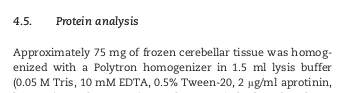
\includegraphics[scale=0.8]{fig/bad_sent_tok_1.png}
\end{center}
As one can see, the beginning of the sentence consists in an overlap of the title of the section and the paragraph following it. 

Another highly represented class of such false sentences is the result of the PDF reader reading the content of data tables in the PDFs.
Here is an example [PMID: 23022093]:
\begin{quote}
Template network Anatomical center of the difference-cluster Coordinates Volume Effect (ml) XYZNOI1 (Medial visual network) NOI2 (Lateral visual network)NOI3 (Somatosensory/auditory network)NOI4 (Sensorimotor network)NOI5 (“Default mode† network)NOI6 (executive/attention/salience network)NOI7 (Left dorsolateral visual stream/working memory)NOI8 (Right dorsolateral visual stream, working memory)Frontal pole 36 91 48 0.51 M > P Hypothalamus 45 59 30 0.49 M > P Cuneus 38 24 50 0.58 M b P Dorsocaudal anterior cingulate 45 66 60 1.32 M b P Cerebellum 55 29 24 1.31 M b P 33 33 23 1.10 M b P Amygdala 33 65 23 1.16 M b P Cuneus 44 26 52 0.85 M b P Precuneus 37 26 59 0.62 M b P Frontal pole 59 86 51 0.47 M b P Supramarginal 74 50 58 0.45 M b P Occipital pole 55 18 32 1.06 M > P Cerebellum 45 42 35 52.67 M b P White matter 53 67 45 3.26 M b P Supramarginal gyrus Right 16 43 51 2.30 M b P Left 75 42 54 0.50 M b P Insula 21 69 36 1.38 M b P Ventricle 42 47 42 0.98 M b P Premotor 38 65 68 0.97 M b P Frontal pole 59 87 48 0.60 M b P Posterior cingulate cortex 45 37 49 8.58 M b P Rostral anterior cingulate 46 90 34 8.52 M b P Frontal pole Right 29 80 59 2.79 M b P Left 58 81 58 2.49 M b P Brainstem 45 60 29 1.94 M b P Fusiform Right 36 26 30 1.58 M b P Left 53 23 28 0.84 M b P Cerebellum 66 27 14 0.97 M b P 54 42 12 0.75 M b P Lateral parietal lobule 65 28 60 0.86 M b P Retrosplenium 39 41 35 0.54 M b P Middle frontal gyrus 71 71 56 0.48 M b P Left caudate 44 63 41 1.01 M b P Dorsal anterior cingulate 45 76 46 0.70 M b P Cerebellum 57 27 17 0.46 M b P Frontal pole, right 30 90 48 0.42 M b P Insula Left 63 71 35 0.41 M b P Right 28 73 29 0.38 M b P Dorsal paracingulate 47 91 44 1.18 M > P Cerebellum 34 23 18 0.74 M > P Frontal pole Left 56 86 53 0.57 M > P Right 24 85 47 1.63 M b P Middle frontal gyrus 32 73 64 1.84 M b P Frontal gyrus Left 65 79 47 16.62 M b P Right 19 78 46 1.98 M b P Left inferior temporal gyrus 72 37 30 2.38 M b P Precuneus 45 26 60 1.46 M b P Superior parietal lobule 68 38 62 0.99 M b P Occipital fusiform 41 22 32 0.73 M b P Left hippocampus 54 55 28 0.67 M b P Retrosplenial cortex 49 42 38 0.41 M b PNOI templates are obtained from independent component analysis as described by Beckmann et al. (2005). 
\end{quote}
while in original PDF it looks like:
\begin{center}
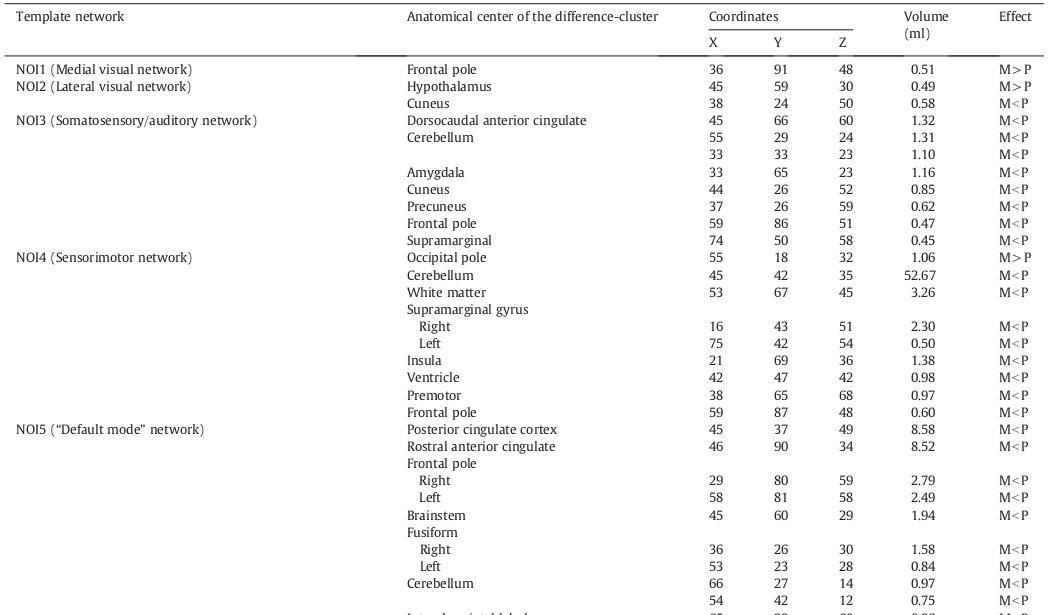
\includegraphics[width=\textwidth]{fig/bad_sent_tok_2.png}
\end{center}
Note that the above example is a good example of the hardness to treat full-text table extracted from PDF documents.
Note that these two classes of error (sentence tokenization problem and table error) are highly correlated ($r = 0.86$). It can be explained by the fact that a table error is a special instance of a sentence tokenization problem. 93\% of the cases where a sentence presents a tokenization problem, the sentence appears to be spanning a data table.
Nevertheless, a quick fix can be deduced from the fact that sentences spanning table content appear to be quite longer than normal sentence. More precisely, the indicator telling whether a
sentence has a length greater than 1000 characters has a 0.768 correlation with the one indicating that a sentence has a table form.
Note that the problems of sentence tokenization is a major problem for our 
extraction. since 71.33\% of the sentences suffers from it. That is, filtering out 
sentences whose length is greater than 1000 charcters appears to be a good 
workaround.

\subsubsection{Bad Chunking}
We talk of bad chunking when a chunk contains non related (syntactically speaking) protein and concentration.
A current pattern in the syntax of scientific literature is the use of enumeration. The co-occurrences of a protein and a concentration 
do not escape this rule. Consider the co-occurrences between biomedical entities and concentration in the following sentence [PMID: 22197517]:

\begin{quote}
Tissues were sonicated in 1\% SDS in TE (pH = 7.4) containing 1 protease inhibitor cocktail (1 mM AEBSF, 0.08 mM aprotinin, 21 mM leupeptin, 36 mM bestatin, 15 mM pepstatin A, and 14 mM E-64).
\end{quote}

Note that the number of co-occurrences grows exponentially with the length of the enumeration. Let $B$ be the set of biomedical entity appearing in the above enumeration.
That is,
$$
B = \{\text{AEBSF, aprotinin, leupeptin, bestatin, pepstatin, E-64}\}
$$
and $C$ the set of all the concentration appearing in the example. That is,
$$
C = \{\text{1 mM, 0.08 mM, 21 mM, 36 mM, 15 mM, 14 mM}\}.
$$

Then, the total number of co-occurrences in the enumeration is $|C\times B|$ when following a naive approach. To solve this misconception, one can argue that, in the model described before, the co-occurrence of a protein and a
concentration is considered as being a relation if the protein and the concentration appears in the same syntaxical chunk. However, in practice, the definition of
chunk provided by the OpenNLP chunker \cite{chunker} contains too much irregularities to assume that any enumeration would be separated on the commas. 

The problem of bad chunking seems to be present in 21\% of our results.
After excluding 
the sentences being badly tokenized from the calculations since it is hard to decide whether a piece of text is properly chunked in those since the concept of chunk only makes sense in a syntactically correct context, 
the resulting sample contains 65.1\% of cases with chunking problem. That is, we decided to add some properties to the definition of chunk, namely
\begin{itemize}
\item a item of an coma-separated enumeration is always one chunk, and
\item pattern of the form '$\langle$a protein mention$\rangle$ ($\langle$a concentration mention$\rangle$)' is always in one chunk.
\end{itemize}
Then, to avoid the combinatorial expansion of the number of co-occurrences, only the high-confidence co-occurrences are kept, namely the co-occurrences with the smallest
distance between their members. Reconsider one of the examples from section
\ref{sec:bannerM} [PMID: 15016809]:
\begin{quote}
The follicular membranes were removed by digestion in Ca2-free OR2 solution ({\color{blue}82.5 mM} NaCl, {\color{blue}2.5 mM} KCl, {\color{blue}1 mM} MgCl , {\color{blue}5 mM} HEPES, 2 pH 7.6) containing {\color{blue}2 mg/ml} {\color{red}collagenase} (Sigma). 
\end{quote}
If one consider all the 5 possibles pc-cooccurrences enclosed by the sentence, it
gets 4 false positives. However, keeping only the nearest-neighbours co-occurrence which contains ``{\color{red}collagenase}'' means keeping only the co-occurrence between it and the closer concentration in the sentence, i.e. ``{\color{blue}2 mg/ml}''. One could argue that this approach can be used among sentences and free us from using chunks. However, notice that a protein and a concentration mentions at both ends of a sentence intuitively tends to be unrelated but could be a nearest-
neighbouts co-occurrence provided no other mention of such kinds exists in the 
sentence. Therefore, we keep our approach to consider pc-cooccurrences among 
chunk, but, in the case where more than one concentration or protein occurs in a 
chunk, we use a nearest-neighbours policy.
\subsubsection{Bad Protein Mentions}
Qualitative analysis of protein estimated mentions reveals two big problems: (1)
when BannerM is run on table, it becomes unpredictable as revealed by these examples of extracted protein estimated mentions:
\begin{itemize}
    \item GR 3 19 F 5 Anisocoria  GR 4 16 M 7 GR 5 35 M 4 Anisocoria  GR 6 48 F 12 Anisocoria GR 7 28 M 3  GR
    \item C9 87 M 17 IV
    \item UI 16 2 79 F 76 3 GD
    \item LB 86 F W 16 Str 
    \item NrA Normal control C-2 80 M 12 NrA Normal control C-3 57 F 8 NrA Normal control C-4 70 M 7 NrA
    \item P Middle frontal gyrus 32 73 64 1.84 M b P Frontal gyrus Left 65 79 47 16.62 M b P Right 19 78 46 1.98 M b P
\end{itemize}
and (2) chemical elements are interpreted as protein mentions such as ``NaCL'' or ``KHPO4''.

The first problem should be overcome by filtering out the text coming from table content using the
length of sentence as explained in section \ref{sec:table_error}.
To limit the number of some obviously non-protein chemical elements BANNER considers as protein mentions, a list-based filter was built based on the more frequent of such confusions. A more long-term efficient approach would have been to use a chemical NER such as OSCAR4 \cite{oscar} to differentiate a protein mentions from chemical ones, but this would have increased the runtime too much considering the time constraint of the project.
